%%%%%%%%%%%%%%%%%%%%%%%%%%%%%%%%

\documentclass[11pt,a4paper]{article}
\usepackage{times}
\usepackage[utf8]{inputenc}
\usepackage[croatian]{babel}
\usepackage[T1]{fontenc} % Latin Modern

%%%%%%%%%%%%%%%%%%%%%%%%%%%%%%%%


%%%%%%%%%%%%%%%%%%%%%%%%%%%%%%%%
%%%%%%%%  MATEMATICKI PAKETI %%%%%%%%%%%
%%%%%%%%%%%%%%%%%%%%%%%%%%%%%%%%

\usepackage{amsmath}
\usepackage{amsfonts}
\usepackage{amssymb}
\usepackage{esvect}

%%%%%%%%%%%%%%%%%%%%%%%%%%%%%%%%

%%%%%%%%%%%%%%%%%%%%%%%%%%%%%%%%
%%%%%%%%%% PAKETI ZA SLIKE  %%%%%%%%%%%%
%%%%%%%%%%%%%%%%%%%%%%%%%%%%%%%%

\usepackage{graphicx}
\usepackage{float}
\usepackage[hidelinks]{hyperref}
\usepackage{caption}
\usepackage{subcaption}
\usepackage{booktabs}

%%%%%%%%%%%%%%%%%%%%%%%%%%%%%%%%

%%%%%%%%%%%%%%%%%%%%%%%%%%%%%%%%
%%%%%%%%%    PRORED 1.5   %%%%%%%%%%%%%%
%%%%%%%%%%%%%%%%%%%%%%%%%%%%%%%%

\renewcommand{\baselinestretch}{1.5}

%%%%%%%%%%%%%%%%%%%%%%%%%%%%%%%%


%%%%%%%%%%%%%%%%%%%%%%%%%%%%%%%%
%%%%%%%%%% TABLICA - ANTUN %%%%%%%%%%%%
%%%%%%%%%%%%%%%%%%%%%%%%%%%%%%%%

\usepackage{array}
\usepackage{multirow}
\newcolumntype{C}[1]{>{\centering\let\newline\\\arraybackslash\hspace{0pt}}m{#1}}
\newcolumntype{L}[1]{>{\raggedright\let\newline\\\arraybackslash\hspace{0pt}}m{#1}}
\newcolumntype{R}[1]{>{\raggedleft\let\newline\\\arraybackslash\hspace{0pt}}m{#1}}
\usepackage{ctable}

%%%%%%%%%%%%%%%%%%%%%%%%%%%%%%%%

%%%%%%%%%%%%%%%%%%%%%%%%%%%%%%%%
%%%%%%%%%% TABLICA - MARTINA %%%%%%%%%%%
%%%%%%%%%%%%%%%%%%%%%%%%%%%%%%%%

\makeatletter
\renewcommand*\env@matrix[1][\arraystretch]{%
  \edef\arraystretch{#1}%
  \hskip -\arraycolsep
  \let\@ifnextchar\new@ifnextchar
  \array{*\c@MaxMatrixCols c}}
\makeatother



%%%% LATEX KOD ZA KORISTENJE TABLICE %%%%
%%% PRIMJER %%%

%\setlength\extrarowheight{1pt}
%\begin{table}[h]
%\centering
%\caption{Tablica s prikazom }
%\label{prva}
%\begin{tabular}{|l|c|}
%\hline
%\textbf{txt} &  \\ \hline 
%txt & txt    \\ 
%txt & txt   \\ \hline
%txt & txt    \\ \hline
%\end{tabular}
%\end{table}

%%%%%%%%%%%%%%%%%%%%%%%%%%%%%%%%


%%%%%%%%%%%%%%%%%%%%%%%%%%%%%%%%
%%%%%%% DIO ZA UNOS ISJECAKA KODA %%%%%%%%
%%%%%%%%%%%%%%%%%%%%%%%%%%%%%%%%

\usepackage{listings}
\usepackage{color}
 
\definecolor{codegreen}{rgb}{0,0.6,0}
\definecolor{codegray}{rgb}{0.5,0.5,0.5}
\definecolor{codepurple}{rgb}{0.58,0,0.82}
 
\lstdefinestyle{mystyle}{   
    commentstyle=\color{codegreen},
    keywordstyle=\color{blue},
    numberstyle=\tiny\color{codegray},
    stringstyle=\color{codepurple},
    basicstyle=\footnotesize,
    breakatwhitespace=false,         
    breaklines=true,                 
    captionpos=b,                    
    keepspaces=true,                 
    numbers=left,                    
    numbersep=5pt,                  
    showspaces=false,                
    showstringspaces=false,
    showtabs=false,                  
    tabsize=1
}
 
\lstset{style=mystyle}

%\lstinputlisting[language=Matlab, firstline=1, lastline=4, numbers=left, frame=single, label={lst:prvi}, caption={Diskretizacija sustava korištenjem Matlaba}, captionpos=b]{peti.m} 

%%%%%%%%%%%%%%%%%%%%%%%%%%%%%%%%


%----------------------------
% za uredjenje stranice
\usepackage[left=2.5cm,right=2.5cm,top=2.5cm,bottom=2.5cm]{geometry}
\usepackage{fancyhdr}
\pagestyle{fancy} 
\lhead{\leftmark}
\rhead{\rightmark}
\usepackage{titlesec} %za točku iza broja sectiona
\titleformat{\section}{\huge\bfseries}{\thetitle.\quad}{0em}{}
\titleformat{\subsection}{\LARGE\bfseries}{\thetitle.\quad}{0em}{}
\titleformat{\subsubsection}{\Large\bfseries}{\thetitle.\quad}{0em}{}
\titleformat{\paragraph}
{\normalfont\large\bfseries}{\thetitle.\quad}{1em}{}
\titlespacing*{\paragraph}
{0pt}{3.25ex plus 1ex minus .2ex}{1.5ex plus .2ex}
\setcounter{secnumdepth}{5}

\usepackage{indentfirst} %uvlacenje prvog paragrafa
% primjer pozivanja sectiona
% \section*{UVOD} \pdfbookmark{UVOD}{section:UVOD}

\usepackage{tocloft}
\usepackage{import}
\usepackage{standalone}
\graphicspath{{figures/}} 

\hypersetup{
  colorlinks   = true, %Colours links instead of ugly boxes
  urlcolor     = black, %Colour for external hyperlinks
  linkcolor    = black, %Colour of internal links
  citecolor   = blue %Colour of citations
}

\usepackage{subcaption}
\usepackage{lscape}
\begin{document}

Robotika je grana tehnologije koja se bavi dizajnom, izradom, upravljanjem i primjenom robota. To je višedisciplinarna znanstvena grana koja objedinjuje znanja iz područja mehanike, elektronike, računarstva i automatike \cite{kova}. Zahvaljujući svakodnevnom napretku tehnologije, te novim postignućima u znanosti, robotika postaje neizostavan dio modernog društva. U posljednjem desetljeću, poseban fokus robotskog istraživanja stavljen je na zračnu robotiku, posebice na multirotorske letjelice. Od posebnog su interesa u istraživanju bespilotnih letjelica autonomne misije, navođenje i upravljanje, koordinacija multi-agentskih sustava letjelica, inovativni dizajn letjelica i drugo. 

\medskip

Potencijalne primjene bespilotnih letjelica dijele se na dvije grupe, vojne i civilne. Prva grupa, \textit{vojne aplikacije}, uključuje akcije kao što su ciljanje i distrakcija, praćenje i izviđanje, sudjelovanje u borbi i logističke primjene, dok druga grupa, \textit{civilne aplikacije}, uključuje akcije kao što su nadgledanje prometa i vremena, vatrogastvo, poljoprivreda, traženje i spašavanje, te istraživanje i razvoj \cite{urs}. Teži se razvoju autonomnih robotskih sustava, sposobnih za rad u izrazito dinamičnim i nedeterminističkim okruženjima.

\medskip

\begin{figure}[H]
	\centering
	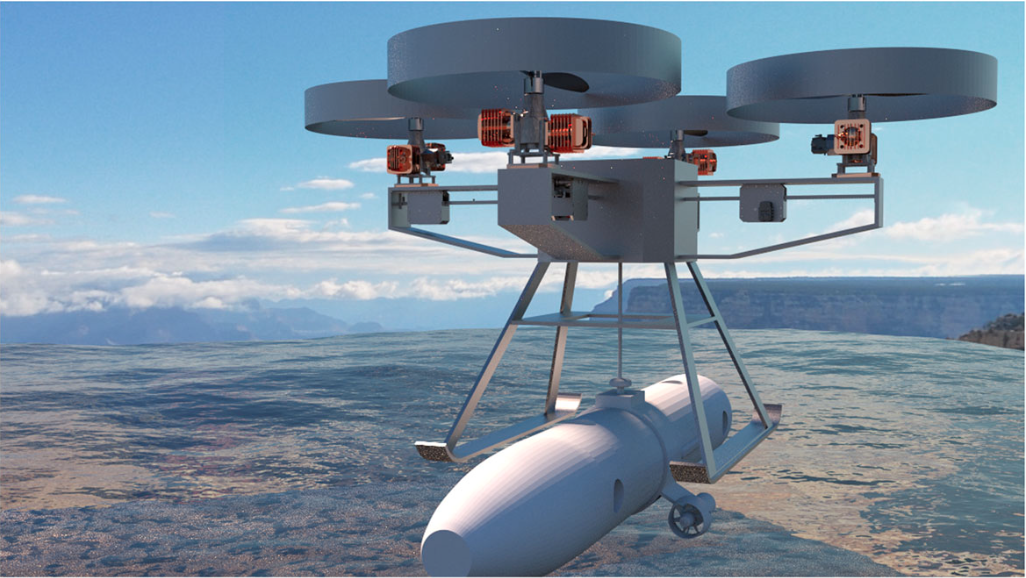
\includegraphics[scale=0.35]{koord}
	\caption{Projekt MORUS - autonomni heterogeni robotski sustav sastavljen od bespilotne letjelice i bespilotne ronilice \cite{haus2}}
	\label{fig:koord}
\end{figure}

Ideja ovog rada proizlazi iz želje za razvojem jednog takvog autonomnog heterogenog robotskog sustava, sastavljenog od bespilotne letjelice i bespilotne ronilice, kao što je prikazano na Slici \ref{fig:koord}. Ovakav robotski sustav služio bi u misijama izviđanja na moru. Znanstvenici s Fakulteta elektrotehnike i računarstva u Zagrebu, na Zavodu za Automatiku i Računalno Inženjerstvo u Laboratoriju za Robotiku i Inteligentne Sustave Upravljanja, pod vodstvom prof. dr. sc. Stjepana Bogdana rade na razvoju jednog ovakvog sustava na projektu pod imenom MORUS. Cilj ovog robotskog sustava je koordinirana akcija između letjelice i ronilice, u kojem bi se ronilica u bazi na obali osigurala za letjelicu, koja bi ju potom prevezla do mjesta na kojoj se obavlja određena misija te ju pustila u more i zatim se vratila u bazu. Po završetku misije letjelica bi otišla po ronilicu, izvukla ju iz mora te vratila na početni položaj, odnosno u bazu \cite{haus2}.


\medskip


Intuitivno je jasno kako su na ovakvu letjelicu postavljeni strogi uvjeti vezani za njezinu nosivost i vrijeme autonomije. Maksimalna masa tereta koju robot može prenijeti i maksimalna brzina gibanja robota ovise o tipu robota i njegovoj primjeni \cite{kova}. Kako bi bespilotna letjelica bila sposobna podići i prenijeti bespilotnu ronilicu na predodređenu lokaciju, treba imati veliku nosivost ($\geq$ 50kg) i vrijeme leta ($\geq$ 60min). Komercijalne bespilotne letjelice ne ispunjavaju zadane kriterije. Njihovo se upravljanje temelji na promjeni brzine rotacije propelera te na korištenju električnih motora. S obzirom na zahtjev veće nosivosti letjelice javila se potreba za razvojem u potpunosti novog sustava upravljanja. U okviru MORUS projekta predlaže se da se električni motori zamjene benzinskim motorima. Benzin, kao spremnik energije, omogućava dulju autonomiju i brže punjenje u odnosu na bateriju. Zbog spore dinamike benzinskih motora uvodi se novi koncept upravljanja temeljen na promjeni centra mase letjelice \cite{haus1}.

\medskip

Benzinski motori, unatoč svojim prednostima, otežavaju testiranje jednog ovakvog sustava. Za pokretanje kompleksnog sustava ovih razmjera potrebna je pomno planirana i vremenski dugotrajna priprema. Sami benzinski motori stvaraju buku i ispušne plinove te zahtijevaju pokretanje na otvorenom. U tu svrhu javlja se potreba za izradom laboratorijske makete letjelice, na kojoj će se testirati svi algoritmi razvijeni za veliku letjelicu. Ovaj rad stoga nastoji doprinijeti dizajnu i razvoju laboratorijske makete letjelice te primijeniti i testirati novi koncept upravljanja bespilotnom letjelicom zasnovan na promjeni centra mase letjelice. 

\end{document}